\section{One-dimensional heat equation}
Now, consider the one-dimensional heat equation:
\begin{equation}
\label{eq:1DHeatEq}
\frac{\partial \phi (x,t)}{\partial t} = D \frac{\partial^2 \phi (x,t)}{\partial^2 x}
\end{equation}
We are interested in the evolution of $\phi(x,t)$  in  time which satisfies equation \ref{eq:1DHeatEq}. The  first step in the finite differences method is to construct a grid with points on which we are interested in solving the equation (this is called discretization, see figure \ref{fig:1d-grid}).

\begin{figure}[ht]\centering
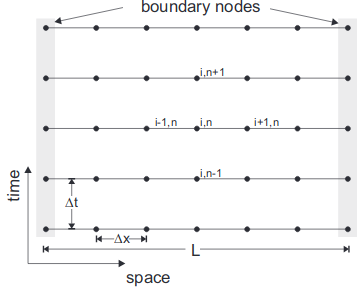
\includegraphics[width=0.5\linewidth]{1d-grid}
\caption{Finite difference discretization of the 1D heat problem}
\label{fig:1d-grid}
\end{figure}

The next step is to replace the continuous derivatives of equation \ref{eq:1DHeatEq} with their finite difference approximations. The derivative of $\phi$ versus time ($\frac{\partial \phi}{\partial t}$) can be approximated with a forward finite difference approximation as
\begin{equation}
\frac{\partial \phi}{\partial t} \approx \frac{\phi^{n+1}_{i}-\phi^{n}_{i}}{t^{n+1}-t^{n}} =\frac{\phi^{n+1}_{i}-\phi^{n}_{i}}{\Delta t}
\label{eq:timeDiscret}
\end{equation}
Here, $n$ represents the time step; and the subscript $i$ refers to the location. Both $n$ and $i$ are integers; $n$ varies from 1 to $n_t$ (total number of time steps) and $i$ varies from 1 to $n_x$ (total number of grid points in x-direction).The spatial derivative of equation \ref{eq:1DHeatEq} is replaced by a central finite difference approximation, i. e. 
\begin{equation}
\frac{\partial^2 \phi}{\partial x^2} = \frac{\partial}{\partial x}\frac{\partial \phi}{\partial x} \approx \frac{\frac{\phi^n_{i+1}-\phi^n_{i}}{\Delta x}-\frac{\phi^n_{i}-\phi^n_{i-1}}{\Delta x}}{\Delta x} = \frac{\phi^n_{i+1}-2\phi^n_{i}+\phi^n_{i-1}}{(\Delta x)^2}
\label{eq:spatialDiscret}
\end{equation}

Substituting equations \ref{eq:timeDiscret} and \ref{eq:spatialDiscret} into equation \ref{eq:1DHeatEq} gives:
\begin{equation}
\frac{\phi^{n+1}_{i}-\phi^{n}_{i}}{\Delta t}=D \frac{\phi^n_{i+1}-2\phi^n_{i}+\phi^n_{i-1}}{(\Delta x)^2}
\label{eq:1DheatDisc}
\end{equation}
Rearrenging the equation \ref{eq:1DheatDisc} gives an evolutionary equation for $\phi$, this method is called \textit{explicit scheme}.
\\
An alternative approach is an \textit{implicit finite difference scheme}, where the spatial derivatives $\frac{\partial^2 \phi}{\partial x^2}$ are evaluated at the new time step. The simplest implicit discretization of equation \ref{eq:1DHeatEq} is
\begin{equation}
\frac{\phi^{n+1}_{i}-\phi^{n}_{i}}{\Delta t}=D \frac{\phi^{n+1}_{i+1}-2\phi^{n+1}_{i}+\phi^{n+1}_{i-1}}{(\Delta x)^2}
\label{eq:1DheatDiscImplicit}
\end{equation}
A \textit{fully implicit} scheme where the time derivative is taken backward can be rearranged so that unknown terms are on the left and known terms are on the right
\begin{equation}
\label{eq:fullyImplicit}
-s \phi^{n+1}_{i+1} + (1+2s) \phi^{n+1}_{i} -s \phi^{n+1}_{i-1}=\phi^{n}_{i}
\end{equation}
where
\begin{equation}
\label{eq:s}
s=\frac{D \Delta t}{(\Delta x)^2}
\end{equation}
Note that in this case we no longer have an explicit relationship for $\phi^{n+1}_{i}$, $\phi^{n+1}_{i-1}$ and $\phi^{n+1}_{i+1}$. Instead, we have to solve a linear system of equations, which is discussed further below.
\\
We solve the heat equation (\ref{eq:1DHeatEq}) on the domain $0 \leq x \leq 1$ subject to the following boundary conditions for fixed temperature
%\begin{equation}

\begin{align}
\label{eq:BC1Dheat}
\phi(x=0)&=\phi_{left} \\
\phi(x=1)&=\phi_{right}
\end{align}
%\end{equation}
Starting with fixed temperature BCs (\ref{eq:BC1Dheat}), the boundary condition on the left boundary gives
\begin{equation}
\label{eq:BC1Dleft}
\phi_1=\phi_{left},
\end{equation}
and the one on the right 
\begin{equation}
\label{eq:BC1Dright}
\phi_{nx}=\phi_{right}.
\end{equation}
\\
Equation \ref{eq:fullyImplicit}, \ref{eq:BC1Dleft} and \ref{eq:BC1Dright} can be written in matrix form as
\begin{equation}
\label{eq:1DlinearSys}
A\vec{x}=\vec{b}.
\end{equation}
Acording to equation \ref{eq:fullyImplicit}, for a five-node grid, for example, the linear system becomes
%\begin{equation}
\begin{align*}
  grid \ point \ \# 1&: \qquad \phi^{n+1}_{1}= \qquad \phi^{n}_{1} &=\phi^{n}_{left} \\
  grid \ point \ \# 2&: -s \phi^{n+1}_{1} + (1+2s)\phi^{n+1}_{2} -s \phi^{n+1}_{3} &= \phi^{n}_{2} \\
  grid \ point \ \# 3&: -s \phi^{n+1}_{2} + (1+2s)\phi^{n+1}_{3} -s \phi^{n+1}_{4} &= \phi^{n}_{3} \\
  grid \ point \ \# 4&: -s \phi^{n+1}_{3} + (1+2s)\phi^{n+1}_{4} -s \phi^{n+1}_{5} &= \phi^{n}_{4} \\
  grid \ point \ \# 5&: \qquad \phi^{n+1}_{5}= \qquad \phi^{n}_{5} &=\phi^{n}_{right} \\
\label{eq:1D5node}
\end{align*}

%\end{equation}
thus the coefficient matrix A is
\begin{equation}
A = \begin{bmatrix}
       1 & 0 & 0 & 0 & 0 \\
	   -s & (1+2s) & -s & 0 & 0 \\
  	   0 & -s & (1+2s) & -s & 0  \\
  	   0 & 0 & -s & (1+2s) & -s  \\  	   
       0 & 0 & 0 & 0 & 1 \\
     \end{bmatrix}
\end{equation}
and vectors $\vec{x}$ and $\vec{b}$ are
\begin{equation}
x=\begin{bmatrix}
\phi^{n+1}_{1} \\ \phi^{n+1}_{2} \\ \phi^{n+1}_{3} \\ \phi^{n+1}_{4} \\ \phi^{n+1}_{5}
\end{bmatrix}
\quad
b=\begin{bmatrix}
\phi_{left} \\ \phi^{n}_{2} \\ \phi^{n}_{3} \\ \phi^{n}_{4} \\ \phi_{right}
\end{bmatrix}
\end{equation}
Note that matrix $A$ will have a unity entry on the diagonal and zero else for each node where Dirichlet (fixed temperature) boundary conditions apply.
\\
In case of the Dirichlet boundary condition, it is better if we get rid of the boundary points ($\phi_{left}$ and $\phi_{right}$) in the solution vector, that is we only take the evolving points. In this case, we have to take the effects of boundaries in a boundary condition vector on the right hand side of the equation \ref{eq:1DlinearSys}, and we can rewrite the equation as:
\begin{equation}
\label{eq:1DlinearSys+B.C.}
A'\vec{x'}=\vec{b'} + \vec{b.c.}
\end{equation} 
where, for a five-node grid the coefficient matrix is:
\begin{equation}
A' = \begin{bmatrix}
	   (1+2s) & -s & 0  \\
  	   -s & (1+2s) & -s \\
  	    0 & -s & (1+2s)   \\  	   
     \end{bmatrix}
\end{equation}
and vectors $\vec{x}$, $\vec{b}$, and $\vec{b.c.}$ are:
\begin{equation}
\vec{x'}=\begin{bmatrix}
 \phi^{n+1}_{2} \\ \phi^{n+1}_{3} \\ \phi^{n+1}_{4}
\end{bmatrix}
\quad
\vec{b'}=\begin{bmatrix}
\phi^{n}_{2} \\ \phi^{n}_{3} \\ \phi^{n}_{4}
\end{bmatrix}
\quad
\vec{b.c.}=s \begin{bmatrix}
\phi_{left} \\ 0 \\ \phi_{right}
\end{bmatrix}
\end{equation}
Linear system \ref{eq:1DlinearSys+B.C.} is like linear system \ref{eq:1DlinearSys}, but only for the evolving points (we have ignored the boundaries).
\\
Matrix $A$ also has an overall peculiar form because most entries off the diagonal are zero. This “sparseness” can be exploited by specialized linear algebra routines, both in terms of storage and speed. By avoiding computations involving zero entries of the matrix, much larger problems can be handled than would be possible if we were to store the full matrix. In particular, the fully implicit FD scheme leads to a “tridiagonal” system of linear equations that can be solved with various well known methods.
Thus solving a PDE is reduced to solve a system of linear equations. There are many methods of numerical solution of linear systems. 
